\section{Introduction}
\begin{figure}[tb]
    \centering
    \begin{tabular}{c c c}
        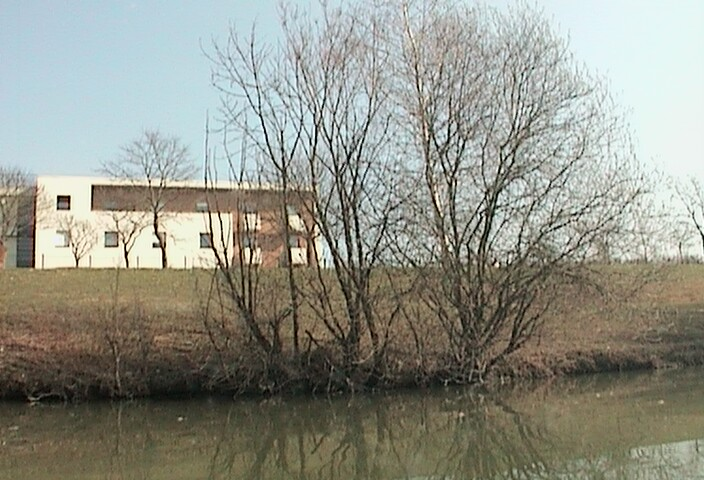
\includegraphics[width=0.3\columnwidth]{siftflow-hard/140314-16329} &
        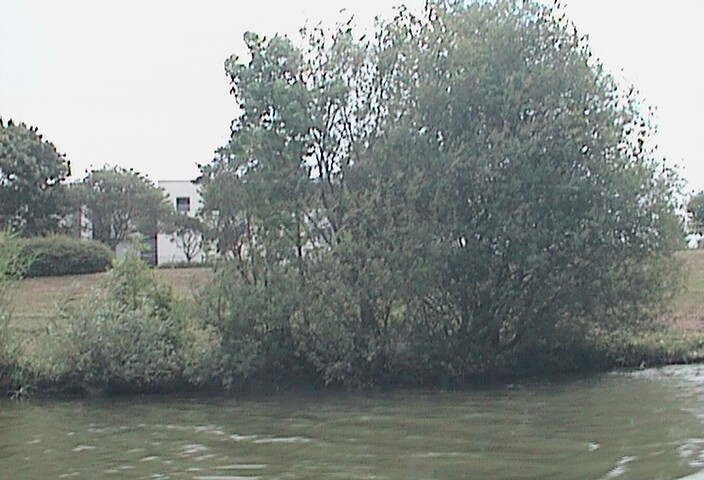
\includegraphics[width=0.3\columnwidth]{siftflow-hard/140625-23223}&
        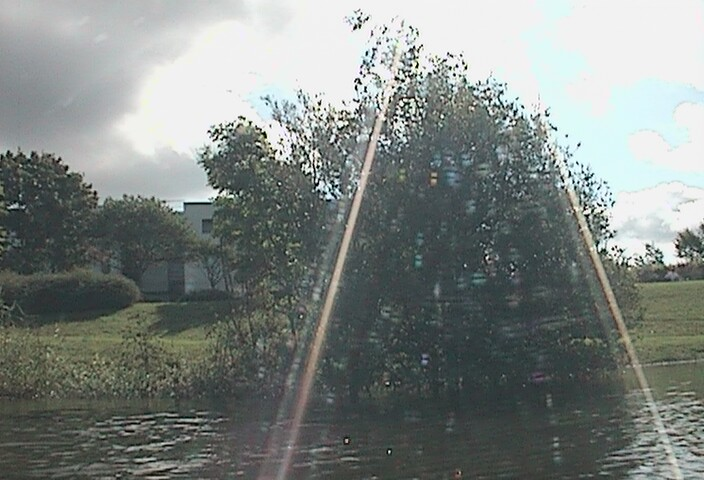
\includegraphics[width=0.3\columnwidth]{siftflow-hard/140812-18224}  \\
        Mar. 14 & June 25 & Aug. 12\\
    \end{tabular}
    \caption{Examples of variation in appearance of a section of the lake shore from winter to summer. The significant variation in the vegetation and lighting conditions makes place recognition particularly challenging.} 
    \label{fig:dataset-hard}
\end{figure}

\label{sec:intro}
Long-term natural environment monitoring using visual inspection is the process
of collecting images of an outdoor landscape over a long duration with respect
to the natural dynamics of this environment. In our case, we are specifically
considering the weekly observation of a lake shore over multiple years using an autonomous boat
programmed to follow the shore at a constant distance while recording images.
As such, our images depict scenes which are combinations of close-up trees, far-away trees, bushes,
lawns, water and sky, with a high level of similarities. Because we work in a
natural setting, this environment is subjected to seasonal changes (trees
blooming, leaves falling, ...), structural changes (cut branch, fallen trees,
mowed lawns) and weather variations impacting the lighting condition, spectrum
and incidence. Figure~\ref{fig:dataset-hard} gives an example of a relatively easy group
of images in our dataset.

To assess the difficulty of interpreting these images, in a
previous work, we evaluated the time required by a human to decide if two
images correspond to the same place albeit at different time of the year. For
some image pairs, our test subjects took more than 30 seconds to confirm their answer.  

One of the challenge of natural environment monitoring is to be able to compare
the appearance of vastly varying outdoor settings with the purpose of at least
detecting unnatural changes (intruders, structural damages, ...) and ideally to
classify changes according to their nature. 

In this context, this paper focuses on the evaluation of deep convolutional
neural networks (CNN, \cite{farabet-pami-13}) applied to images of natural environments
subjected to large seasonal variations. The task we set ourselves has three
stages. In a first stage, we evaluate the ability of a CNN to recognize a place
independently of the seasonal and lighting changes. This problem is framed as a
classification task where each class is a location around our lake shore and a
standard network structure can be used. In a
second stage, we now consider a CNN trained to predict the pose (or view point)
of the camera (2D position and heading) using an adapted network structure
suitable for a regression task. Finally, in a third stage, we evaluate the
quality of the internal representation learned by the convolutional layers of
the CNN to describe a place independently of its seasonal appearance as well as
the generalizability of the resulting features. This third stage is important
for the potential of this internal representation to be used to detect changes
with respect to a season-invariant representation of a place. 

In summary, this paper contribution is two-fold. First, it introduces a
relatively unique long-term natural environment monitoring dataset to the
computer vision community.  Secondly and more importantly, this paper is a
benchmark on the performance of CNN for the very particular task of processing
images of natural environments subjected to large seasonal changes and natural
lighting conditions variation. 

All the results presented in this paper have been trained using the Caffe
library~\cite{jia2014caffe} with a default network structure where possible.  

% Check {\tt bmvc\_guidelines.pdf} for the original text.
% - Experimentation of deep learning technique for localization in a natural environment
% - Goal: obtaining a seasonal invariant and light invariant representation of natural environment images
% - Unique dataset 
% - Two different approaches: classification and regression
% - Starting point: testing a network (CaffeNet) which performs well on classification task for well known datasets such as ImageNet.
% 
% - Classification: ...
% - Regression: we try to learn the model that match the image to the GPS coordinates which can allow to identify a place robustly.
